\documentclass[main.tex]{subfiles}

\begin{document}
	
	\section{Постановка задачи}
	Поставлена задача линейного программирования:
	\begin{equation}\label{eq:initial}
	\left\{
	\begin{array}{ll} 
	x_1-2x_2+2x_3 \le 6\\
	x_1+2x_2+x_3+x_4=24\\
	2x_1+x_2-4x_3+x_4=30\\
	-x_1+4x_2-2x_4 \ge -6\\
	x_1 \ge 0
	\end{array}
	\right.
	\end{equation}
	$$ 8x_1 + 8x_2 - 4x_3 - 2x_4 \longrightarrow min $$
	\begin{enumerate}
		\item Привести задачу к виду, необходимому для применения симплекс-метода.
		\item Построить к данной задаче двойственную и также привести к виду, необходимому для применения симплекс-метода.
		\item Решить обе задачи симплекс-методом с выбором начального приближения методом искусственного базиса.
		\item Решить обе задачи методом перебора крайних точек.
		\item Разработать схему восстановления прямой задачи по решению двойственной.
	\end{enumerate}
	Алгоритмы, требуемые для решения задачи, реализовать в таком виде, чтобы их можно было использовать в качестве подпрограмм в следующих лабораторных работах.
	\section{Исследование применимости метода}
	Алгоритм симплекс-метода, приведённый в пособии \cite{petuh} и описанный ниже, применим к задачам линейного программирования на нахождение минимума. Метод работает с задачами в канонической форме при всяких вещественных значениях компонент $A \in \mathds{R}_{m\times n}, b \in \mathds{R}_m, c \in R_n$ с условием: матрица $A$ имеет ранг $m$ (следовательно, существует хотя бы один опорный вектор).\\
	После приведения задачи (\ref{eq:initial}) (или двойственной к ней) к каноническому виду получается система с матрицей $ 4 \times 9 $ ранга $4$, следовательно, условие выполнено.\\
	
	\newpage
	\section{Описание алгоритмов}
	\subsection{Алгоритм перевода из общей в каноническую форму}
	\textbf{Вход}: система
	% TODO написать вид системы
	\begin{enumerate}
		\item Проверяем знаки в системе
		\item Если <<$\le$>>, то к левой части добавляем $w[i]$, если <<$\ge$>>, то из левой части вычитаем $w[i]$, $w[i]\ge0$.
		\item Знаки неравенства в системе заменяем на равенство.
		\item Производим замену переменных: если $x[i]\le0$, то $x'[i]=-x[i]\ge0$; если $x[i]$ любого знака, то $x[i]=u[i]-v[i]$, $v[i],u[i] \ge 0$.
	\end{enumerate}
	\subsection{Алгоритм построения двойственной задачи}
	Для простоты алгоритма будем рассматривать задачу минимума:
	\begin{equation}\label{eq:maxproblem}
	\begin{array}{ll}
	(x[N],c[N])\longrightarrow \min_{x[N]}, x[N] \in S, x[N] \ge 0\\
	S :=\{x[N]|A[M,N]\cdot x[N] \gtreqless b[M]\}, x[N] \ge 0
	\end{array}
	\end{equation}
	Если перед нами стоит задача максимума, то домножим вектор коэффициентов матрицы цели на $-1$.
	\begin{enumerate}
		\item Транспонируем заданную матрицу $А$
		\item Новый вектор коэффицентов, стоящий в системе справа, равен вектору коэффициентов функции цели (\ref{eq:maxproblem}).
		\item Новый вектор коэффициентов функции цели равен вектору коэффицентов, стоящему в системе (\ref{eq:maxproblem}) справа.
		\item Если ограничение на $x[i]\ge0$, то $i$-ая строка новой системы имеет знак <<$\ge$>>.
		Если нет ограничения на знак, то $i$-ая строка новой системы имеет знак <<$=$>>.
		\item Если ограничение $i$-ой строки в исходной системе <<$\ge$>> (тк рассматриваем задачу  минимума), то ограничение на знак новой переменной $y[i]\ge0$.
		Если ограничение $i$-ой строки в исходной системе <<$=$>>, то $y[i]$ любого знака.
		\item Если исходная задача на поиск минимума, то двойственная на поиск максимума.
	\end{enumerate}
	\subsection{Алгоритм симплекс-метода и связанные процедуры}
	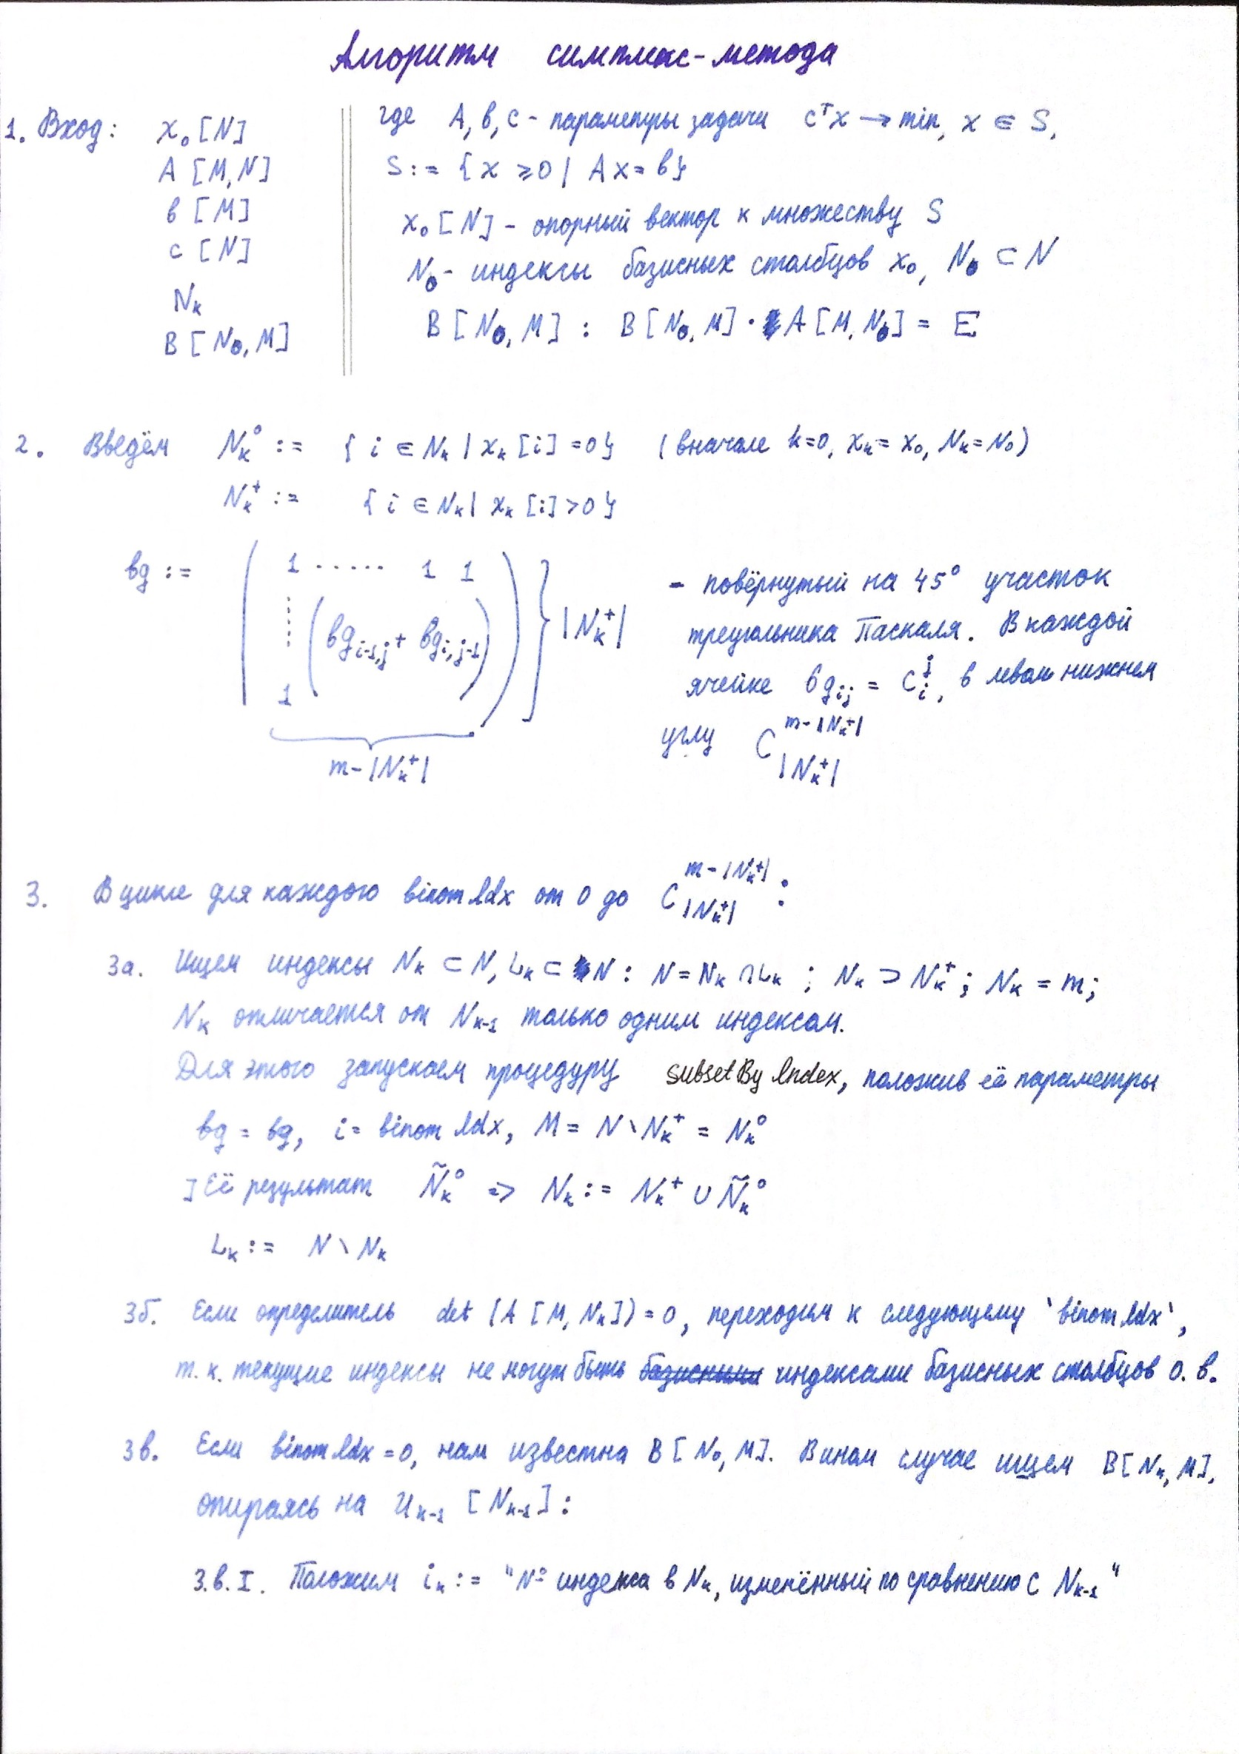
\includepdf[pages=-]{simplexEtcWritten.pdf}
	\subsection{Алгоритм перебора опорных векторов}
	Опорные векторы можно искать прямо по определению, перебирая все возможные базисы и находя соответствующие ненулевые коэффициенты из решения СЛАУ. Множества входящих в базис столбцов будем определять с помощью метода \textit{subsetByIndex}, описанной в предыдущем разделе. Также будем пользоваться процедурой \textit{inv}, описываемой в следующем разделе, для нахождения обратной матрицы при решении СЛАУ.\\
	
	\SetKwRepeat{Do}{do}{while}
	\begin{algorithm}[H]\label{points}
		\KwData{$A[M,N], b[M], c[N]$ -- параметры задачи линейного программирования, поставленной в канонической форме\; $m=|M|, n=|N|$}
		\KwResult{опорный вектор $x_*[N]$, минимизирующий целевую функцию $(x[N],c[N])$}
		инициализация матрицы $bg[N,M]$ биномиальных коэффициентов\;
		$V:=\emptyset$ -- будущий список опорных векторов\;
		\For{$i$ в диапазоне $\{0;C_m^n\}$}{
			$N_k := $  subsetByIndex($i$,$bg$)\;
			\If{$|det(A[M,N_k])| > eps$}{
				$x[N_k]:=$ inv($A[M,N_k], b[M]$)\;
				Дополняем нулями до $x[N]$\;
				Добавляем $x[N]$ в $V$\;
			}
		}
		Выбираем $x_*$  -- любой вектор из $V$\;
		\For{$v \in V$}{
			\If{$(v,c) < (x_*,c)$}{
				$x_*:=v$\;
			}
		}
		
		\caption{Метод перебора опорных векторов решения задачи линейного программирования в канонической форме}
	\end{algorithm}
	
	\subsection {Алгоритм восстановления решения прямой(двойственной) задачи по решению двойственной(прямой)}
	Рассмотрим пару двойственных задач, образованную основной задачей линейного программирования и двойственной к ней:
	\begin{itemize}
		\item Прямая (исходная) задача:
		\begin{equation}\label{eq:primal}
		\begin{array}{ll}
		F = (x[N],c[N])\longrightarrow \max_{x[N]}, x[N] \in S\\
		S =\{x[N]|A[M,N]\cdot x[N] = b[M], x[N] \ge 0\}
		\end{array}
		\end{equation}
		\item Двойственная к ней  задача:
		\begin{equation}\label{eq:dual}
		\begin{array}{ll}
		F_{dual} = (y[M],b[M])\longrightarrow \min_{y[M]}, y[M] \in S_{dual}\\
		S_{dual} =\{y[M]|A^{T}[N,M]\cdot y[M] \le c[N]\}
		\end{array}
		\end{equation}
	\end{itemize}
	Каждая из задач (\ref{eq:primal}) и (\ref{eq:dual}) фактически является самостоятельной задачей линейного программирования и может быть решена независимо от другой. Однако при нахождении оптимального плана одной из задач при помощи симплекс метода или метода искусственного базиса находится решение и другой задачи.
	\newline Пусть: \begin{itemize}
		\item $x^{*}$ -- найденный оптимальный план  задачи (\ref{eq:primal});
		\item $P_{i_1}, P_{i_2}, \ldots, P_{i_m}$ -- базис, определяющий план; \item $C_{basis} := (c_{i_1}, c_{i_2}, \ldots, c_{i_m})$ -- вектор-строка, составленная из коэффициентов при неизвестных в целевой функции задачи (\ref{eq:primal});
		\item $P^{-1}$ - матрица, обратная матрице $P$, составленной из базисных векторов.
	\end{itemize}
	Тогда будем находить решение прямой задачи в соответствии с теоремой \cite{akulich}: \begin{theorem}Если основная задача линейного программирования имеет оптимальный план $x^{*}$, то $y^{*} = C_{basis}\cdot P^{-1}$ является оптимальным планом двойственной задачи.\end{theorem}
	
	Теперь, помня о том, что задачи (\ref{eq:primal}) и (\ref{eq:dual}) двойственны друг к другу, можем решать любую из них и находить оптимальный план для парной с затратами лишь на обращение матрицы из базисных векторов и на умножение этой матрицы на вектор $C_{basis}$.
	
	\section{Результаты решения задачи}
	Симплекс метод для задачи (\ref{eq:initial}) дал нам оптимальный план $\widetilde{x_{*}}^T = (0., -3.5, -0.5, 31.5)$.\newline
	Метод перебора крайних точек дал нам решение $\widetilde{\widetilde{x_{*}}}^T = (0., -3.5, -0.5, 31.5)$.\newline
	При этом точное решение задачи $x_{*}^T = (0., -\frac{7}{2}, -\frac{1}{2}, \frac{63}{2})$ - его можно получить, например, при решении в дробях системы из строки (6) алгоритма перебора крайних точек (\ref{points}).\newline
	Сравнив результаты, полученные при использовании исследуемых методов, между собой и с точным решением, можем сделать вывод, что абсолютная погрешность при нашей реализации очень хорошая. Такую ситуацию имеем за счет того, что достаточно малые числа компьютер просто не хранит. Неточности, попадающие в область машинного нуля, нивелируются.
	
	\section{Оценка достоверности полученного результата}
	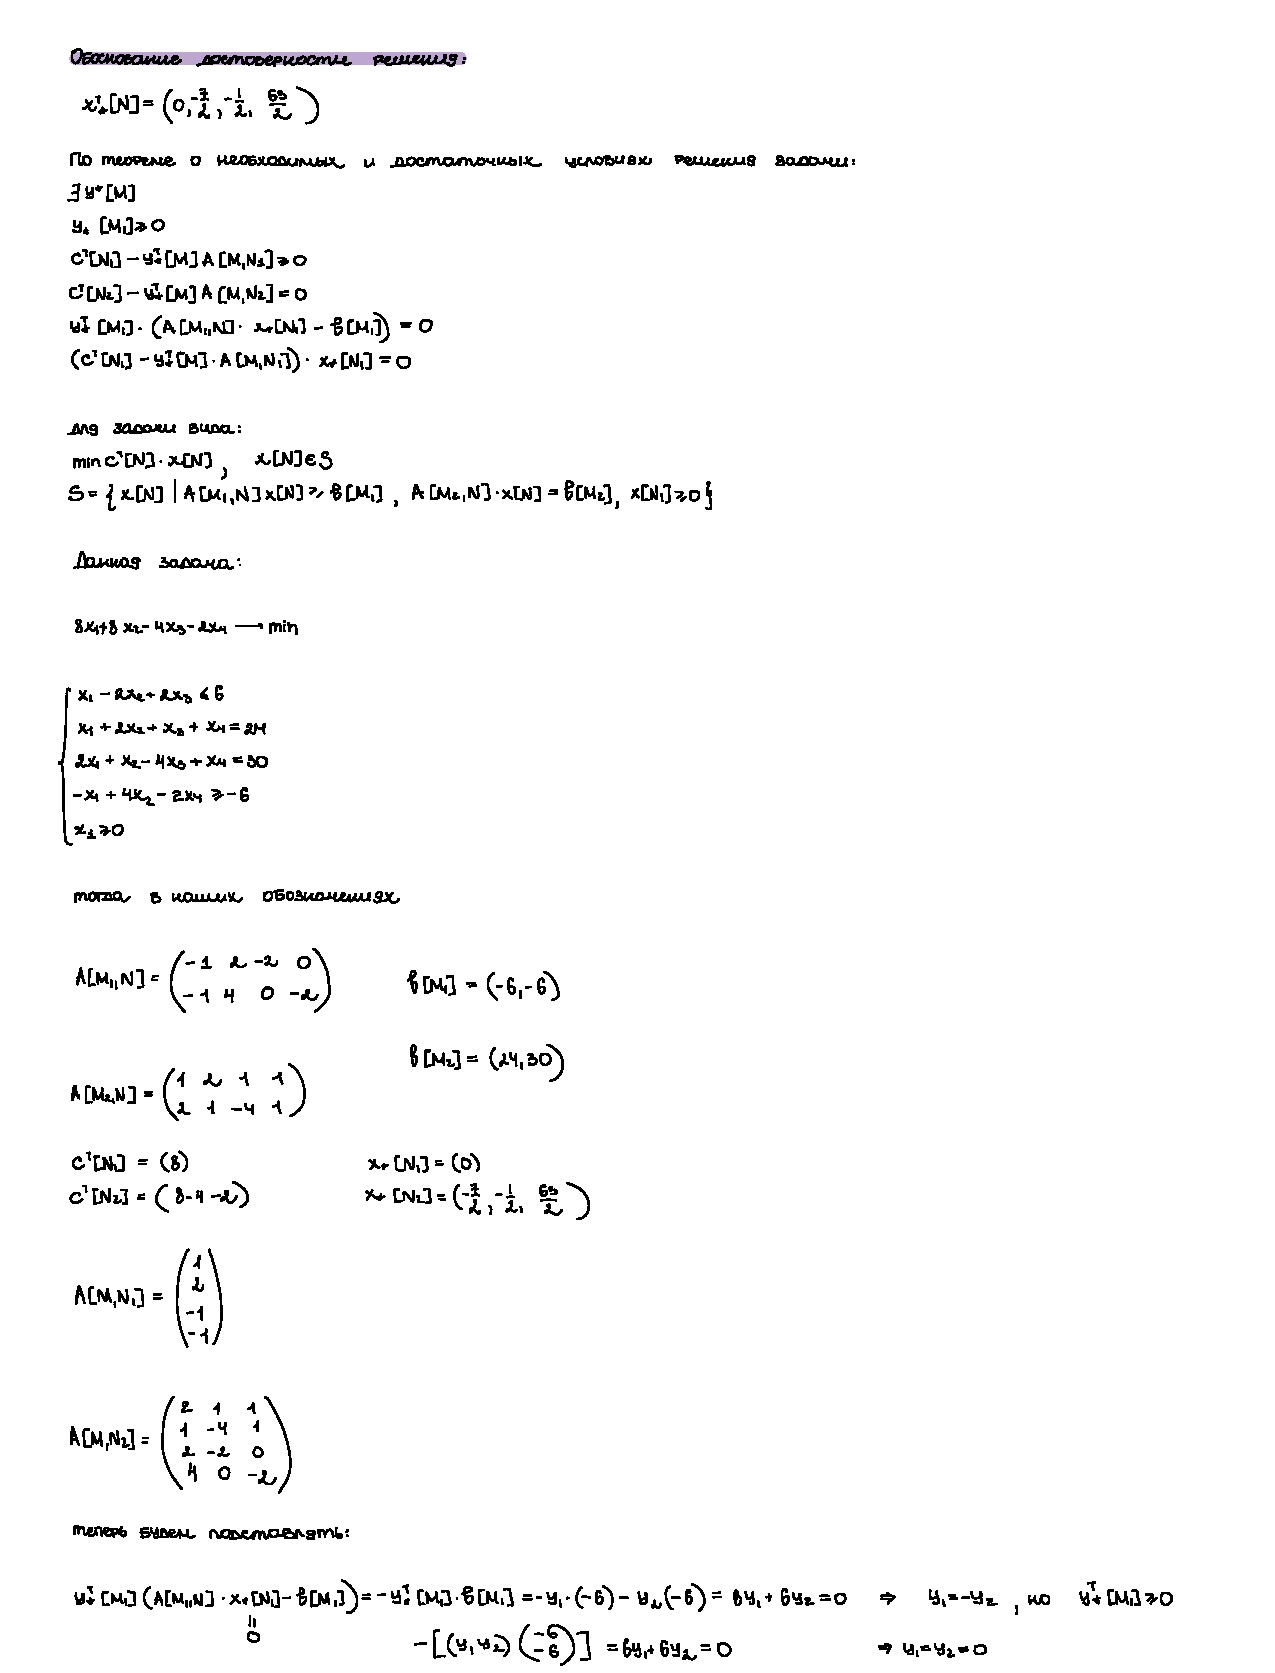
\includepdf[pages=-]{solutionCredibility.pdf}
	\begin{thebibliography}{99}
		\bibitem{petuh} Петухов Л. В. Методы оптимизации. Задачи выпуклого программирования: учеб. пособие / Л. В. Петухов, Г. А. Серёгин, Е. А. Родионова. -- СПб.: Изд-во Политехн. ун-та, 2014. -- 99 с.
		\bibitem{akulich} Акулич И.Л. Математическое программирование в примерах и задачах: учеб. пособие. -- СПб.: Изд-во 'Лань', 2011. -- 352с.: ил.
	\end{thebibliography}
	
	
\end{document}
